\documentclass{beamer}[10]
\usepackage{pgf}
\usepackage{beamerthemesplit}
\usepackage{array}
\usepackage{wrapfig}
\usepackage{varwidth}
%\usepackage{enumitem}
\usepackage{listings}
\lstset{language=bash,
	basicstyle=\ttfamily\scriptsize,		
	keywordstyle=\color{blue}\ttfamily,
	morekeywords={peter@kbpet},
	alsoletter={:~$},
	morekeywords=[2]{peter@kbpet:},
	keywordstyle=[2]{\color{red}},
	literate={\$}{{\textcolor{red}{\$}}}1 
	{:}{{\textcolor{red}{:}}}1
	{~}{{\textcolor{red}{\textasciitilde}}}1,
	breaklines=true,
	numbers=none,
	numbersep=5pt,
	stepnumber=1
}
\usepackage{algorithm,algpseudocode}
\usepackage{hyperref}
%\usepackage{pdfpc-commands}
\usepackage{pgfpages}

\usepackage{tikz}
\usetikzlibrary{er,positioning}
\usepackage{float}
\usepackage{subcaption}
\usepackage{xcolor}
\usepackage[acronym,sort=def]{glossaries}

%\usepackage{natbib}
\bibliographystyle{apalike}

\definecolor{kugreen}{RGB}{50,93,61}
\definecolor{kugreenlys}{RGB}{132,158,139}
\definecolor{kugreenlyslys}{RGB}{173,190,177}
\definecolor{kugreenlyslyslys}{RGB}{214,223,216}
\definecolor{kublue}{RGB}{0,101,163}
\definecolor{kubluelys}{RGB}{132,158,139}
\definecolor{kubluelyslys}{RGB}{173,190,177}
\definecolor{kubluelyslyslys}{RGB}{214,223,216}
\setbeamercovered{transparent}
\mode<presentation>
\usetheme[numbers,totalnumber,compress,sidebarshades]{PaloAlto}
%\setbeamertemplate{footline}[frame number]

\usecolortheme[named=kublue]{structure}
\useinnertheme{circles}
\usefonttheme[onlymath]{serif}
\setbeamercovered{transparent}
\setbeamertemplate{blocks}[rounded][shadow=true]
%\setbeameroption{show notes on second screen}
%\setbeameroption{show notes}

\logo{
\includegraphics[width=1.5cm]{gfx/eth_logo_kurz_pos}}
\title{Map Fusion for Collaborative UAV SLAM}
\subtitle{Map Fusion for Collaborative UAV SLAM}
\author{Andreas Ziegler}
\institute{V4RL \\ ETH Zürich}
\date{12th of January 2017}

\newcommand{\setlistspacing}[2]{\def\@ld{#1}\expandafter\def\csname
	@list\romannumeral\@ld \endcsname{\leftmargin\csname
		leftmargin\romannumeral\@ld \endcsname
		\topsep    #2
		\parsep    0\p@   \@plus\p@
		\itemsep   #2}}
\makeatother

\newacronym{slam}{SLAM}{Simultaneous Localisation and Mapping}
\newacronym{uav}{UAV}{Unmanned aerial vehicle}

\newacronym{kf}{KF}{key frame}
\newacronym{kfm}{KFM}{key frame match}

\newacronym{ba}{BA}{bundle adjustment}
\newacronym{gba}{GBA}{global bundle adjustment}
\newacronym{pgo}{PGO}{pose graph optimization}

\newacronym{lm}{LM}{Levenberg-Marquardt}
\newacronym{dl}{DL}{Powell's dog leg}

\makeglossaries

\begin{document}

\frame { \frametitle{Semester Project}
	\begin{center}
	\LARGE Semester Project \\
	- \\
	Map Fusion for Collaborative UAV SLAM\\
	- \\
	\includegraphics*[height=0.6cm]{gfx/eth_logo_kurz_pos.eps} \hfill
	\includegraphics*[height=0.6cm]{gfx/v4rl_logo} \hfill
	\includegraphics*[height=0.6cm]{gfx/asl_logo_right.pdf}
	\end{center}
}

\frame { \frametitle{Contents}
	\tableofcontents
}

\section{Introduction}
\frame{\tableofcontents[currentsection]}

\frame{ \frametitle{Introduction}
	\begin{itemize}
	\visible<1-5>{
  \item \glspl{slam} is one of the most important challenges for robots to be autonomous.
	}
	\visible<2-5>{
  \item For a team of \glspl{uav} collaboratively performing tasks, a common map is required
  }
  \visible<3-5>{
  \item To build a common map from the maps of the \glspl{uav}, the maps need to be merged
  }
	\visible<4-5>{
	\item To merge two maps, the alignment of them has to be found
	}
	\visible<5>{	
	\item Redundant information should be removed to achieve a better performance
	}
	\end{itemize}
}
\note[enumerate]
{
	\item for many interactive systems, especially for robotic systems interacting with humans.
	\item any such tracking approach has to balance plasticity versus drift, in particular when an object should be re-detected after loss of tracking.
}

\section{Motivation}
\frame{\tableofcontents[currentsection]}

\frame{ \frametitle{Motivation}
	\begin{itemize}
  \visible<1-4>{
\item Using multiple \glspl{kfm} to guarantee no false map merging
  }
  \visible<2-4>{
  \item Using multiple \glspl{kfm} to obtain an optimal map alignment
  }
  \visible<3-4>{
  \item Perform \gls{kf} culling to remove redundant information as bundle adjustment complexity grows with the number of \gls{kf}
  }
  \visible<4>{
  \item A multi agent SLAM system based on ORB-SLAM2 should be extended
  }
  \end{itemize}
  \visible<3>{\cite{Mur-Artal2015}}
  \visible<4>{\cite{Mur-Artal2015,Mur-Artal2016}}
}

\frame{ \frametitle{Acronyms}
  %\printglossaries
  \printglossary[nonumberlist,type=\acronymtype]
}

\section{Map merging}
\frame{\tableofcontents[currentsection]}

\subsection{Approaches}
\frame{	\frametitle{Map merging - Old approach}
   Old approach:
	\begin{itemize}
    \item As soon as a \glspl{kfm} was detected, maps were merged
	\end{itemize}
}

\frame{
  \frametitle{Map merging - New approach}
  New approach:
	\begin{enumerate}
  \pause
  \item After a \gls{kfm} is found skip $m$ \gls{kf} before processing the next \gls{kfm}
  \pause
  \item Wait for $n$ \glspl{kfm}
  \pause
  \item Merge the two maps with the transformation of one of the \glspl{kfm}
  \pause
  \item Fuse map points in the ($n-1$) \glspl{kfm}
  \pause
  \item \acrfull{pgo} over essential graph
  \pause
  \item \acrfull{gba}
	\end{enumerate}
}

\frame{
  \frametitle{Map merging - New approach}
  \only<1>{
  Find $n$ \acrfull{kfm}
  \begin{center}
  \begin{tikzpicture}
    \coordinate (A1) at (0, 3);
    \coordinate (A1MP1) at (-0.5, 3.5);
    \coordinate (A1MP2) at (0, 3.75);
    \coordinate (A1MP3) at (0.5, 3.5);

    \coordinate (AB11) at (4/3, 3);
    \coordinate (AB11MP1) at (-0.25+4/3, 3.25);
    \coordinate (AB11MP2) at (4/3, 3.5);
    \coordinate (AB11MP3) at (0.25+4/3, 3.25);

    \coordinate (AB12) at (8/3, 3);
    \coordinate (AB12MP1) at (-0.25+8/3, 3.25);
    \coordinate (AB12MP2) at (8/3, 3.5);
    \coordinate (AB12MP3) at (0.25+8/3, 3.25);

    \coordinate (B1) at (4, 3);
    \coordinate (B1MP1) at (3.2, 3.15);
    \coordinate (B1MP2) at (3.4, 3.6);
    \coordinate (B1MP3) at (3.9, 3.5);

    \coordinate (BC11) at (4, 4);
    \coordinate (BC11MP1) at (3.75, 4.25);
    \coordinate (BC11MP2) at (3.5, 4.0);
    \coordinate (BC11MP3) at (3.75, 3.75);

    \coordinate (BC12) at (4, 5);
    \coordinate (BC12MP1) at (3.75, 5.25);
    \coordinate (BC12MP2) at (3.5, 5.0);
    \coordinate (BC12MP3) at (3.75, 4.75);

    \coordinate (C1) at (4, 6);
    \coordinate (C1MP1) at (3.5, 6.5);
    \coordinate (C1MP2) at (3.25, 6.0);
    \coordinate (C1MP3) at (3.5, 5.5);

    \coordinate (A2) at (0, 0);
    \coordinate (A2MP1) at (-0.5, 0.5);
    \coordinate (A2MP2) at (0, 0.75);
    \coordinate (A2MP3) at (0.5, 0.5);

    \coordinate (AB21) at (2, 0);
    \coordinate (AB21MP1) at (1.75, 0.25);
    \coordinate (AB21MP2) at (2, 0.5);
    \coordinate (AB21MP3) at (2.25, 0.25);

    \coordinate (AB22) at (4, 0);
    \coordinate (AB22MP1) at (3.75, 0.25);
    \coordinate (AB22MP2) at (4, 0.5);
    \coordinate (AB22MP3) at (4.25, 0.25);

    \coordinate (AB23) at (6, 0);
    \coordinate (AB23MP1) at (5.75, 0.25);
    \coordinate (AB23MP2) at (6, 0.5);
    \coordinate (AB23MP3) at (6.25, 0.25);

    \coordinate (B2) at (8, 0);
    \coordinate (B2MP1) at (7.2, 0.15);
    \coordinate (B2MP2) at (7.4, 0.6);
    \coordinate (B2MP3) at (7.9, 0.5);

    \coordinate (BC21) at (8, 1.5);
    \coordinate (BC21MP1) at (7.75, 1.75);
    \coordinate (BC21MP2) at (7.5, 1.5);
    \coordinate (BC21MP3) at (7.75, 1.25);

    \coordinate (BC22) at (8, 3);
    \coordinate (BC22MP1) at (7.75, 3.25);
    \coordinate (BC22MP2) at (7.5, 3.0);
    \coordinate (BC22MP3) at (7.75, 2.75);

    \coordinate (BC23) at (8, 4.5);
    \coordinate (BC23MP1) at (7.75, 4.75);
    \coordinate (BC23MP2) at (7.5, 4.5);
    \coordinate (BC23MP3) at (7.75, 4.25);

    \coordinate (C2) at (8, 6);
    \coordinate (C2MP1) at (7.5, 6.5);
    \coordinate (C2MP2) at (7.25, 6.0);
    \coordinate (C2MP3) at (7.5, 5.5);

    \node [fill=orange!70, circle,inner sep=3pt, text width=0.1mm] at (A1) {};
    \node [fill=green!70, circle,inner sep=2pt, text width=0.1mm] at (A1MP1) {};
    \node [fill=green!70, circle,inner sep=2pt, text width=0.1mm] at (A1MP2) {};
    \node [fill=green!70, circle,inner sep=2pt, text width=0.1mm] at (A1MP3) {};
    \draw [green!50, dashed, line width=0.05cm] (A1) to (A1MP1);
    \draw [green!50, dashed, line width=0.05cm] (A1) to (A1MP2);
    \draw [green!50, dashed, line width=0.05cm] (A1) to (A1MP3);

    \node [fill=orange!30, circle,inner sep=2pt, text width=0.1mm] at (AB11) {};
    \node [fill=green!30, circle,inner sep=1pt, text width=0.1mm] at (AB11MP1) {};
    \node [fill=green!30, circle,inner sep=1pt, text width=0.1mm] at (AB11MP2) {};
    \node [fill=green!30, circle,inner sep=1pt, text width=0.1mm] at (AB11MP3) {};
    \draw [green!50, dashed, line width=0.025cm] (AB11) to (AB11MP1);
    \draw [green!50, dashed, line width=0.025cm] (AB11) to (AB11MP2);
    \draw [green!50, dashed, line width=0.025cm] (AB11) to (AB11MP3);

    \node [fill=orange!30, circle,inner sep=2pt, text width=0.1mm] at (AB12) {};
    \node [fill=green!30, circle,inner sep=1pt, text width=0.1mm] at (AB12MP1) {};
    \node [fill=green!30, circle,inner sep=1pt, text width=0.1mm] at (AB12MP2) {};
    \node [fill=green!30, circle,inner sep=1pt, text width=0.1mm] at (AB12MP3) {};
    \draw [green!50, dashed, line width=0.025cm] (AB12) to (AB12MP1);
    \draw [green!50, dashed, line width=0.025cm] (AB12) to (AB12MP2);
    \draw [green!50, dashed, line width=0.025cm] (AB12) to (AB12MP3);

    \node [fill=orange!70, circle, inner sep=3pt, text width=0.1mm] at (B1) {};
    \node [fill=green!70, circle, inner sep=2pt, text width=0.1mm] at (B1MP1) {};
    \node [fill=green!70, circle, inner sep=2pt, text width=0.1mm] at (B1MP2) {};
    \node [fill=green!70, circle, inner sep=2pt, text width=0.1mm] at (B1MP3) {};
    \draw [green!50, dashed, line width=0.05cm] (B1) to (B1MP1);
    \draw [green!50, dashed, line width=0.05cm] (B1) to (B1MP2);
    \draw [green!50, dashed, line width=0.05cm] (B1) to (B1MP3);

    \node [fill=orange!30, circle, inner sep=2pt, text width=0.1mm] at (BC11) {};
    \node [fill=green!30, circle,inner sep=1pt, text width=0.1mm] at (BC11MP1) {};
    \node [fill=green!30, circle,inner sep=1pt, text width=0.1mm] at (BC11MP2) {};
    \node [fill=green!30, circle,inner sep=1pt, text width=0.1mm] at (BC11MP3) {};
    \draw [green!50, dashed, line width=0.025cm] (BC11) to (BC11MP1);
    \draw [green!50, dashed, line width=0.025cm] (BC11) to (BC11MP2);
    \draw [green!50, dashed, line width=0.025cm] (BC11) to (BC11MP3);

    \node [fill=orange!30, circle, inner sep=2pt, text width=0.1mm] at (BC12) {};
    \node [fill=green!30, circle,inner sep=1pt, text width=0.1mm] at (BC12MP1) {};
    \node [fill=green!30, circle,inner sep=1pt, text width=0.1mm] at (BC12MP2) {};
    \node [fill=green!30, circle,inner sep=1pt, text width=0.1mm] at (BC12MP3) {};
    \draw [green!50, dashed, line width=0.025cm] (BC12) to (BC12MP1);
    \draw [green!50, dashed, line width=0.025cm] (BC12) to (BC12MP2);
    \draw [green!50, dashed, line width=0.025cm] (BC12) to (BC12MP3);

    \node [fill=orange!70, circle,inner sep=3pt, text width=0.1mm] at (C1) {};
    \node [fill=green!70, circle, inner sep=2pt, text width=0.1mm] at (C1MP1) {};
    \node [fill=green!70, circle, inner sep=2pt, text width=0.1mm] at (C1MP2) {};
    \node [fill=green!70, circle, inner sep=2pt, text width=0.1mm] at (C1MP3) {};
    \draw [green!50, dashed, line width=0.05cm] (C1) to (C1MP1);
    \draw [green!50, dashed, line width=0.05cm] (C1) to (C1MP2);
    \draw [green!50, dashed, line width=0.05cm] (C1) to (C1MP3);

    \node [fill=blue!70, circle,inner sep=3pt, text width=0.1mm] at (A2) {};
    \node [fill=green!70, circle,inner sep=2pt, text width=0.1mm] at (A2MP1) {};
    \node [fill=green!70, circle,inner sep=2pt, text width=0.1mm] at (A2MP2) {};
    \node [fill=green!70, circle,inner sep=2pt, text width=0.1mm] at (A2MP3) {};
    \draw [green!50, dashed, line width=0.05cm] (A2) to (A2MP1);
    \draw [green!50, dashed, line width=0.05cm] (A2) to (A2MP2);
    \draw [green!50, dashed, line width=0.05cm] (A2) to (A2MP3);

    \node [fill=blue!30, circle,inner sep=2pt, text width=0.1mm] at (AB21) {};
    \node [fill=green!30, circle,inner sep=1pt, text width=0.1mm] at (AB21MP1) {};
    \node [fill=green!30, circle,inner sep=1pt, text width=0.1mm] at (AB21MP2) {};
    \node [fill=green!30, circle,inner sep=1pt, text width=0.1mm] at (AB21MP3) {};
    \draw [green!50, dashed, line width=0.025cm] (AB21) to (AB21MP1);
    \draw [green!50, dashed, line width=0.025cm] (AB21) to (AB21MP2);
    \draw [green!50, dashed, line width=0.025cm] (AB21) to (AB21MP3);

    \node [fill=blue!30, circle,inner sep=2pt, text width=0.1mm] at (AB22) {};
    \node [fill=green!30, circle,inner sep=1pt, text width=0.1mm] at (AB22MP1) {};
    \node [fill=green!30, circle,inner sep=1pt, text width=0.1mm] at (AB22MP2) {};
    \node [fill=green!30, circle,inner sep=1pt, text width=0.1mm] at (AB22MP3) {};
    \draw [green!50, dashed, line width=0.025cm] (AB22) to (AB22MP1);
    \draw [green!50, dashed, line width=0.025cm] (AB22) to (AB22MP2);
    \draw [green!50, dashed, line width=0.025cm] (AB22) to (AB22MP3);

    \node [fill=blue!30, circle,inner sep=2pt, text width=0.1mm] at (AB23) {};
    \node [fill=green!30, circle,inner sep=1pt, text width=0.1mm] at (AB23MP1) {};
    \node [fill=green!30, circle,inner sep=1pt, text width=0.1mm] at (AB23MP2) {};
    \node [fill=green!30, circle,inner sep=1pt, text width=0.1mm] at (AB23MP3) {};
    \draw [green!50, dashed, line width=0.025cm] (AB23) to (AB23MP1);
    \draw [green!50, dashed, line width=0.025cm] (AB23) to (AB23MP2);
    \draw [green!50, dashed, line width=0.025cm] (AB23) to (AB23MP3);

    \node [fill=blue!70, circle,inner sep=3pt, text width=0.1mm] at (B2) {};
    \node [fill=green!70, circle,inner sep=2pt, text width=0.1mm] at (B2MP1) {};
    \node [fill=green!70, circle,inner sep=2pt, text width=0.1mm] at (B2MP2) {};
    \node [fill=green!70, circle,inner sep=2pt, text width=0.1mm] at (B2MP3) {};
    \draw [green!50, dashed, line width=0.05cm] (B2) to (B2MP1);
    \draw [green!50, dashed, line width=0.05cm] (B2) to (B2MP2);
    \draw [green!50, dashed, line width=0.05cm] (B2) to (B2MP3);

    \node [fill=blue!30, circle,inner sep=2pt, text width=0.1mm] at (BC21) {};
    \node [fill=green!30, circle,inner sep=1pt, text width=0.1mm] at (BC21MP1) {};
    \node [fill=green!30, circle,inner sep=1pt, text width=0.1mm] at (BC21MP2) {};
    \node [fill=green!30, circle,inner sep=1pt, text width=0.1mm] at (BC21MP3) {};
    \draw [green!50, dashed, line width=0.025cm] (BC21) to (BC21MP1);
    \draw [green!50, dashed, line width=0.025cm] (BC21) to (BC21MP2);
    \draw [green!50, dashed, line width=0.025cm] (BC21) to (BC21MP3);

    \node [fill=blue!30, circle,inner sep=2pt, text width=0.1mm] at (BC22) {};
    \node [fill=green!30, circle,inner sep=1pt, text width=0.1mm] at (BC22MP1) {};
    \node [fill=green!30, circle,inner sep=1pt, text width=0.1mm] at (BC22MP2) {};
    \node [fill=green!30, circle,inner sep=1pt, text width=0.1mm] at (BC22MP3) {};
    \draw [green!50, dashed, line width=0.025cm] (BC22) to (BC22MP1);
    \draw [green!50, dashed, line width=0.025cm] (BC22) to (BC22MP2);
    \draw [green!50, dashed, line width=0.025cm] (BC22) to (BC22MP3);
    
    \node [fill=blue!30, circle,inner sep=2pt, text width=0.1mm] at (BC23) {};
    \node [fill=green!30, circle,inner sep=1pt, text width=0.1mm] at (BC23MP1) {};
    \node [fill=green!30, circle,inner sep=1pt, text width=0.1mm] at (BC23MP2) {};
    \node [fill=green!30, circle,inner sep=1pt, text width=0.1mm] at (BC23MP3) {};
    \draw [green!50, dashed, line width=0.025cm] (BC23) to (BC23MP1);
    \draw [green!50, dashed, line width=0.025cm] (BC23) to (BC23MP2);
    \draw [green!50, dashed, line width=0.025cm] (BC23) to (BC23MP3);

    \node [fill=blue!70, circle,inner sep=3pt, text width=0.1mm] at (C2) {};
    \node [fill=green!70, circle, inner sep=2pt, text width=0.1mm] at (C2MP1) {};
    \node [fill=green!70, circle, inner sep=2pt, text width=0.1mm] at (C2MP2) {};
    \node [fill=green!70, circle, inner sep=2pt, text width=0.1mm] at (C2MP3) {};
    \draw [green!50, dashed, line width=0.05cm] (C2) to (C2MP1);
    \draw [green!50, dashed, line width=0.05cm] (C2) to (C2MP2);
    \draw [green!50, dashed, line width=0.05cm] (C2) to (C2MP3);

    \draw [orange!50, line width=0.05cm] (A1) to (B1);
    \draw [orange!50, line width=0.05cm] (B1) to (C1);
    \draw [blue!50, line width=0.05cm] (A2) to (B2);
    \draw [blue!50, line width=0.05cm] (B2) to (C2);

    \draw [red!50, line width=0.05cm, dashed] (A1) to (A2);
    \draw [red!50, line width=0.05cm, dashed] (B1) to (B2);
    \draw [red!50, line width=0.05cm, dashed] (C1) to (C2);

    \node[draw] at (0.5, 5.3)
    {
    \scriptsize
    \begin{tabular}{cl}
      \tikz\node[fill=orange!70, circle,inner sep=3pt, text width=0.1mm] {}; \tikz\node[fill=blue!70, circle,inner sep=3pt, text width=0.1mm] {}; & key frames of a match \\
      \tikz\node[fill=orange!30, circle,inner sep=2pt, text width=0.1mm] {}; \tikz\node[fill=blue!30, circle,inner sep=2pt, text width=0.1mm] & skipped key frames \\
      \tikz\node [fill=green!70, circle, inner sep=2pt, text width=0.1mm] {}; \tikz\node[fill=green!30, circle,inner sep=1pt, text width=0.1mm] {}; & map points
    \end{tabular}
    };

  \end{tikzpicture}
  \end{center}
  }
  \only<2>{
  Merge the two maps and fuse map points
  \begin{center}
  \begin{tikzpicture}
    \coordinate (A1) at (0, 0.25);
    \coordinate (A1MP1) at (-0.5, 0.75);
    \coordinate (A1MP2) at (0, 1.0);
    \coordinate (A1MP3) at (0.5, 0.75);

    \coordinate (AB11) at (4/3, 0.25);
    \coordinate (AB11MP1) at (-0.25+4/3, 0.5);
    \coordinate (AB11MP2) at (4/3, 0.75);
    \coordinate (AB11MP3) at (0.25+4/3, 0.5);

    \coordinate (AB12) at (8/3, 0.25);
    \coordinate (AB12MP1) at (-0.25+8/3, 0.5);
    \coordinate (AB12MP2) at (8/3, 0.75);
    \coordinate (AB12MP3) at (0.25+8/3, 0.5);

    \coordinate (B1) at (4, 0.25);
    \coordinate (B1MP1) at (3.2, 0.15);
    \coordinate (B1MP2) at (3.4, 0.6);
    \coordinate (B1MP3) at (3.9, 0.5);

    \coordinate (BC11) at (4, 4.75/3);
    \coordinate (BC11MP1) at (3.75, 4.75/3 + 0.25);
    \coordinate (BC11MP2) at (3.5, 4.75/3);
    \coordinate (BC11MP3) at (3.75, 4.75/3 - 0.25);

    \coordinate (BC12) at (4, 4.75/1.5);
    \coordinate (BC12MP1) at (3.75, 4.75/1.5 + 0.25);
    \coordinate (BC12MP2) at (3.5, 4.75/1.5);
    \coordinate (BC12MP3) at (3.75, 4.75/1.5 - 0.25);

    \coordinate (C1) at (4, 5);
    \coordinate (C1MP1) at (3.5, 5.5);
    \coordinate (C1MP2) at (3.25, 5.0);
    \coordinate (C1MP3) at (3.5, 4.5);

    \coordinate (A2) at (0, 0);

    \coordinate (B2) at (5.5, 0);

    \coordinate (BC21) at (5.5, 4.75/4);
    \coordinate (BC21MP1) at (5.25, 4.75/4 + 0.25);
    \coordinate (BC21MP2) at (5.0, 4.75/4);
    \coordinate (BC21MP3) at (5.25, 4.75/4 - 0.25);

    \coordinate (BC22) at (5.5, 4.75/2);
    \coordinate (BC22MP1) at (5.25, 4.75/2 + 0.25);
    \coordinate (BC22MP2) at (5.0, 4.75/2);
    \coordinate (BC22MP3) at (5.25, 4.75/2 - 0.25);

    \coordinate (BC23) at (5.5, 3*4.75/4);
    \coordinate (BC23MP1) at (5.25, 3*4.75/4 + 0.25);
    \coordinate (BC23MP2) at (5.0, 3*4.75/4);
    \coordinate (BC23MP3) at (5.25, 3*4.75/4 - 0.25);

    \coordinate (C12) at (4.5, 5.0);
    \coordinate (C2) at (5.5, 5);

    \node [fill=orange!70, circle,inner sep=2pt, text width=0.1mm] at (A1) {};
    \node [fill=green!30, circle,inner sep=2pt, text width=0.1mm] at (A1MP1) {};
    \node [fill=green!30, circle,inner sep=2pt, text width=0.1mm] at (A1MP2) {};
    \node [fill=green!30, circle,inner sep=2pt, text width=0.1mm] at (A1MP3) {};
    \draw [green!50, line width=0.05cm] (A1) to (A1MP1);
    \draw [green!50, line width=0.05cm] (A1) to (A1MP2);
    \draw [green!50, line width=0.05cm] (A1) to (A1MP3);

    \node [fill=orange!30, circle,inner sep=1.5pt, text width=0.1mm] at (AB11) {};
    \node [fill=green!30, circle,inner sep=1pt, text width=0.1mm] at (AB11MP1) {};
    \node [fill=green!30, circle,inner sep=1pt, text width=0.1mm] at (AB11MP2) {};
    \node [fill=green!30, circle,inner sep=1pt, text width=0.1mm] at (AB11MP3) {};
    \draw [green!50, dashed, line width=0.025cm] (AB11) to (AB11MP1);
    \draw [green!50, dashed, line width=0.025cm] (AB11) to (AB11MP2);
    \draw [green!50, dashed, line width=0.025cm] (AB11) to (AB11MP3);

    \node [fill=orange!30, circle,inner sep=1.5pt, text width=0.1mm] at (AB12) {};
    \node [fill=green!30, circle,inner sep=1pt, text width=0.1mm] at (AB12MP1) {};
    \node [fill=green!30, circle,inner sep=1pt, text width=0.1mm] at (AB12MP2) {};
    \node [fill=green!30, circle,inner sep=1pt, text width=0.1mm] at (AB12MP3) {};
    \draw [green!50, dashed, line width=0.025cm] (AB12) to (AB12MP1);
    \draw [green!50, dashed, line width=0.025cm] (AB12) to (AB12MP2);
    \draw [green!50, dashed, line width=0.025cm] (AB12) to (AB12MP3);

    \node [fill=orange!70, circle,inner sep=2pt, text width=0.1mm] at (B1) {};
    \node [fill=green!30, circle, inner sep=2pt, text width=0.1mm] at (B1MP1) {};
    \node [fill=green!30, circle, inner sep=2pt, text width=0.1mm] at (B1MP2) {};
    \node [fill=green!30, circle, inner sep=2pt, text width=0.1mm] at (B1MP3) {};
    \draw [green!50, line width=0.05cm] (B1) to (B1MP1);
    \draw [green!50, line width=0.05cm] (B1) to (B1MP2);
    \draw [green!50, line width=0.05cm] (B1) to (B1MP3);

    \node [fill=orange!30, circle, inner sep=1.5pt, text width=0.1mm] at (BC11) {};
    \node [fill=green!30, circle,inner sep=1pt, text width=0.1mm] at (BC11MP1) {};
    \node [fill=green!30, circle,inner sep=1pt, text width=0.1mm] at (BC11MP2) {};
    \node [fill=green!30, circle,inner sep=1pt, text width=0.1mm] at (BC11MP3) {};
    \draw [green!50, dashed, line width=0.025cm] (BC11) to (BC11MP1);
    \draw [green!50, dashed, line width=0.025cm] (BC11) to (BC11MP2);
    \draw [green!50, dashed, line width=0.025cm] (BC11) to (BC11MP3);

    \node [fill=orange!30, circle, inner sep=1.5pt, text width=0.1mm] at (BC12) {};
    \node [fill=green!30, circle,inner sep=1pt, text width=0.1mm] at (BC12MP1) {};
    \node [fill=green!30, circle,inner sep=1pt, text width=0.1mm] at (BC12MP2) {};
    \node [fill=green!30, circle,inner sep=1pt, text width=0.1mm] at (BC12MP3) {};
    \draw [green!50, dashed, line width=0.025cm] (BC12) to (BC12MP1);
    \draw [green!50, dashed, line width=0.025cm] (BC12) to (BC12MP2);
    \draw [green!50, dashed, line width=0.025cm] (BC12) to (BC12MP3);

    \node [fill=orange!70, circle,inner sep=2pt, text width=0.1mm] at (C1) {};
    \node [fill=green!30, circle, inner sep=2pt, text width=0.1mm] at (C1MP1) {};
    \node [fill=green!30, circle, inner sep=2pt, text width=0.1mm] at (C1MP2) {};
    \node [fill=green!30, circle, inner sep=2pt, text width=0.1mm] at (C1MP3) {};
    \draw [green!50, line width=0.05cm] (C1) to (C1MP1);
    \draw [green!50, line width=0.05cm] (C1) to (C1MP2);
    \draw [green!50, line width=0.05cm] (C1) to (C1MP3);

    \node [fill=blue!70, circle,inner sep=2pt, text width=0.1mm] at (A2) {};
    \draw [green!50, line width=0.05cm] (A2) to (A1MP1);
    \draw [green!50, line width=0.05cm] (A2) to (A1MP2);
    \draw [green!50, line width=0.05cm] (A2) to (A1MP3);

    \node [fill=blue!70, circle,inner sep=2pt, text width=0.1mm] at (B2) {};
    \draw [green!50, line width=0.05cm] (B2) to (B1MP1);
    \draw [green!50, line width=0.05cm] (B2) to (B1MP2);
    \draw [green!50, line width=0.05cm] (B2) to (B1MP3);

    \node [fill=blue!30, circle,inner sep=1.5pt, text width=0.1mm] at (BC21) {};
    \node [fill=green!30, circle,inner sep=1pt, text width=0.1mm] at (BC21MP1) {};
    \node [fill=green!30, circle,inner sep=1pt, text width=0.1mm] at (BC21MP2) {};
    \node [fill=green!30, circle,inner sep=1pt, text width=0.1mm] at (BC21MP3) {};
    \draw [green!50, dashed, line width=0.025cm] (BC21) to (BC21MP1);
    \draw [green!50, dashed, line width=0.025cm] (BC21) to (BC21MP2);
    \draw [green!50, dashed, line width=0.025cm] (BC21) to (BC21MP3);

    \node [fill=blue!30, circle,inner sep=1.5pt, text width=0.1mm] at (BC22) {};
    \node [fill=green!30, circle,inner sep=1pt, text width=0.1mm] at (BC22MP1) {};
    \node [fill=green!30, circle,inner sep=1pt, text width=0.1mm] at (BC22MP2) {};
    \node [fill=green!30, circle,inner sep=1pt, text width=0.1mm] at (BC22MP3) {};
    \draw [green!50, dashed, line width=0.025cm] (BC22) to (BC22MP1);
    \draw [green!50, dashed, line width=0.025cm] (BC22) to (BC22MP2);
    \draw [green!50, dashed, line width=0.025cm] (BC22) to (BC22MP3);

    \node [fill=blue!30, circle,inner sep=1.5pt, text width=0.1mm] at (BC23) {};
    \node [fill=green!30, circle,inner sep=1pt, text width=0.1mm] at (BC23MP1) {};
    \node [fill=green!30, circle,inner sep=1pt, text width=0.1mm] at (BC23MP2) {};
    \node [fill=green!30, circle,inner sep=1pt, text width=0.1mm] at (BC23MP3) {};
    \draw [green!50, dashed, line width=0.025cm] (BC23) to (BC23MP1);
    \draw [green!50, dashed, line width=0.025cm] (BC23) to (BC23MP2);
    \draw [green!50, dashed, line width=0.025cm] (BC23) to (BC23MP3);

    \node [fill=blue!70, circle,inner sep=2pt, text width=0.1mm] at (C2) {};
    \draw [green!50, line width=0.05cm] (C2) to (C1MP1);
    \draw [green!50, line width=0.05cm] (C2) to (C1MP2);
    \draw [green!50, line width=0.05cm] (C2) to (C1MP3);

    \draw [orange!50, line width=0.05cm] (A1) to (B1);
    \draw [orange!50, line width=0.05cm] (B1) to (C1);
    \draw [blue!50, line width=0.05cm] (A2) to (B2);
    \draw [blue!50, line width=0.05cm] (B2) to (C2);

    \draw [red!50, line width=0.05cm, dashed] (A1) to (A2);
    \draw [red!50, line width=0.05cm, dashed] (B1) to (B2);
    \draw [red!50, line width=0.05cm, dashed] (C1) to (C2);

    \node[draw] at (0.25, 4.0)
    {
    \scriptsize
    \begin{tabular}{cl}
      \tikz\node[fill=orange!70, circle,inner sep=2pt, text width=0.1mm] {}; \tikz\node[fill=blue!70, circle,inner sep=2pt, text width=0.1mm] {}; & key frames of a match \\
      \tikz\node[fill=orange!30, circle,inner sep=1.5pt, text width=0.1mm] {}; \tikz\node[fill=blue!30, circle,inner sep=1.5pt, text width=0.1mm] & skipped key frames \\
      \tikz\node [fill=green!70, circle, inner sep=2pt, text width=0.1mm] {}; \tikz\node[fill=green!30, circle,inner sep=1pt, text width=0.1mm] {}; & map points
    \end{tabular}
    };
  \end{tikzpicture}
  \end{center}
  }
}

\subsection{Results}
\frame{
  \frametitle{Map merging - Results - skipping of \gls{kf}}
  \textcolor{green}{green}: Covisibility graph of first map\\ \textcolor{yellow}{yellow}: Covisibility graph of second map\\ \textcolor{red}{red}: Covisibility between the \glspl{kfm}
  \begin{figure}[H]
    \centering
    \subcaptionbox{1 \gls{kf} skipped after a \gls{kfm}}{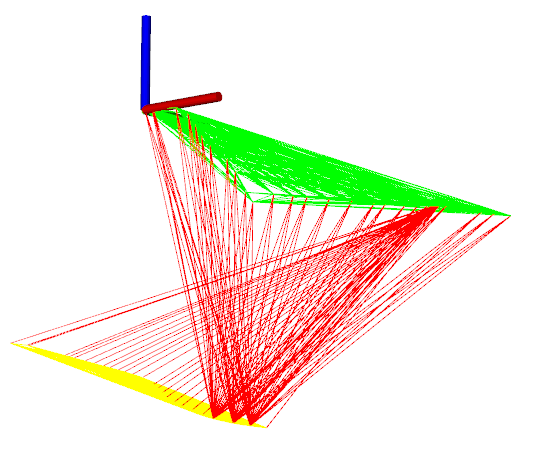
\includegraphics[scale=0.21]{gfx/covgraph_minHits_5_skip_1}}
    \subcaptionbox{10 \gls{kf} skipped after a \gls{kfm}}{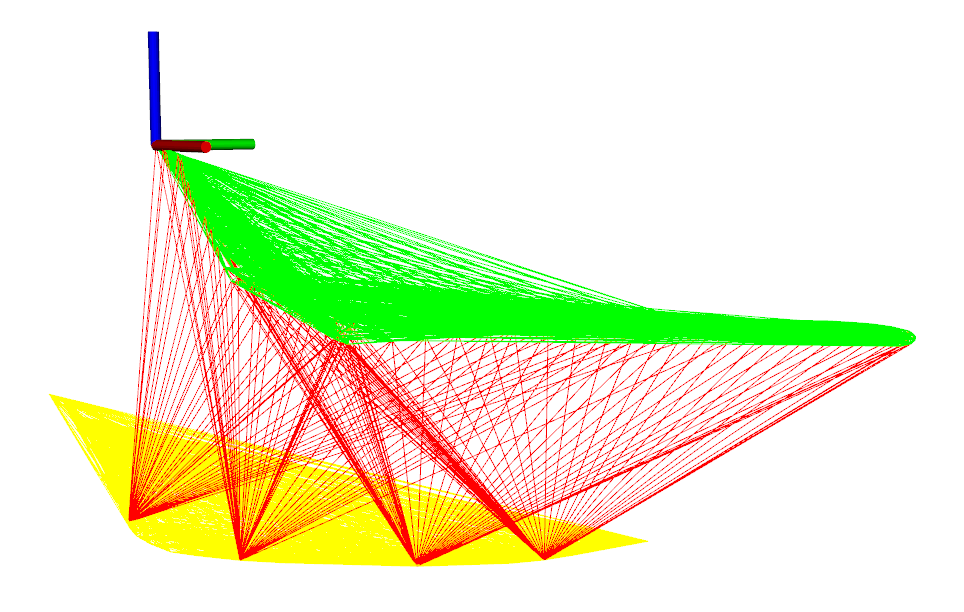
\includegraphics[scale=0.17]{gfx/covgraph_minHits_5_skip_10}}
  \end{figure}
}

\frame{
  \frametitle{Map merging - Results - Reduction of drift}
  \begin{figure}[H]
    \centering
    \subcaptionbox{original approach}{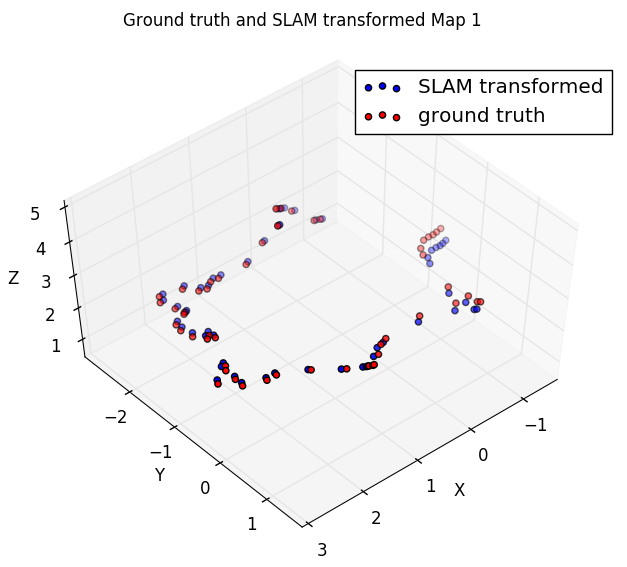
\includegraphics[scale=0.225]{gfx/m1_skf0_cut}}
    \subcaptionbox{new approach}{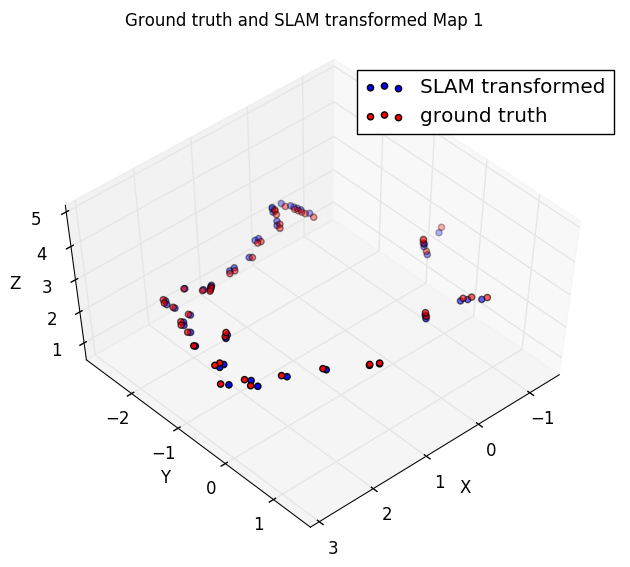
\includegraphics[scale=0.225]{gfx/m10_skf10_cut}}
  \end{figure}

}

\section{Culling}
\frame{\tableofcontents[currentsection]}

\frame{
  \frametitle{Culling - Remove redundant \gls{kf}}
  \begin{itemize}
    \visible<1-4>{
    \item Remove redundant \gls{kf} after $n$ \glspl{kfm} were found
    }
    \visible<2-4>{
    \item{Performs culling for every \gls{kfm} separately
    }
      \begin{itemize}
        \visible<3-4>{
        \item Check \textcolor{red}{\glspl{kf}} which are directly connected to one of the \glspl{kf} of the \gls{kfm} by the \textcolor{blue}{co-visibility graph}
        }
        \visible<4>{
        \item If x\% of the observations of a \gls{kf} are also observed in another \gls{kf}, this \gls{kf} will be deleted.
        }
      \end{itemize}
    }

  \end{itemize}

  \visible<3-4>{
  \begin{center}
    \begin{tikzpicture}[auto]
      \node[entity] (key frame match) {kf match}
        [grow=down,sibling distance=4.5cm]
        child {node[entity] (child 1) {kf, map 1}
          [grow=down,sibling distance=1.2cm]
          child {node[entity,minimum size=1cm] {kf 1}}
          child {node[entity,minimum size=1cm] {kf 2}}
          child {node[entity,minimum size=1cm] {kf $k$}}}
        child {node[entity] {kf, map 2}
          [grow=down,sibling distance=1.2cm]
          child {node[entity,minimum size=1cm] {kf 1}}
          child {node[entity,minimum size=1cm] {kf 2}}
          child {node[entity,minimum size=1cm] {kf $l$}}};

      \draw[blue,thick,dashed] (-2.25,-2.25) ellipse (1.5 and 0.5);
      \draw[blue,thick,dashed] (2.25,-2.25) ellipse (1.5 and 0.5);
      \draw[red,thick,dashed] (0,-2.25) ellipse (5 and 1.5);
    \end{tikzpicture}
  \end{center}
  }
}

\subsection{Results}
\frame{
  \frametitle{Culling - Results}
  \visible<1-2>{
  \acrfull{pgo}\\
  \acrfull{gba}\\

  \begin{table}[ht!]
  \begin{center}
  \begin{tabular}{c|c|c|c|c}
    Culling &  \# matches & \# \glspl{kf} skipped & \acrshort{pgo} [ms] & \acrshort{gba} [ms] \\ 
    \hline 
    No & 1 & 0 &142.25 & 163.89 \\
    Yes & 1 & 0 & 42.01 & 72.33 \\
    No & 10 & 10 & 532.28 & 3659.48 \\
    Yes & 10 & 10 & 178.83 & 1098.37 \\
    %\hline 
  \end{tabular}
  \end{center}
  \caption{Time measurements of \gls{pgo} and \gls{gba} without and with culling.}
  \label{tab:results_time}
  \end{table}
  }

  \visible<2>{
    \begin{block}{}
      Performance increases significantly when culling is enabled
    \end{block}
  }
}

\frame{
  \frametitle{Culling - Results}
  \visible<1-2>{
  \begin{table}[ht!]
  \begin{center}
  \begin{tabular}{c|c|c|c}
    Culling &  \# matches & \# \glspl{kf}s skipped & \textit{rmse} [m] \\ 
    \hline 
    No & 1 & 0 & 0.1310 \\
    Yes & 1 & 0 & 0.2187 \\
    No & 10 & 10 & 0.0961 \\
    Yes & 10 & 10 & 0.0965 \\
    %\hline 
  \end{tabular}
  \end{center}
  \caption{\textit{rmse} without and with culling.}
  \label{tab:results_rmse}
  \end{table}
  }

  \visible<2>{
    \begin{block}{}
      Accuracy gets worser if not enough information is available.\\No problem with multiple \acrfull{kfm}.
    \end{block}
  }
}

\section{Dog leg opt.}
\frame{\tableofcontents[currentsection]}

\frame{
  \frametitle{Use dog leg optimizer - Idea}
  \begin{block}{}
  Considerable computational benefits can be gained by substituting the \acrfull{lm} algorithm in the implementation of \acrfull{ba} with a variant of \acrfull{dl} non-linear least squares technique \cite{Lourakis2005}
  \end{block}
}

\frame{
  \frametitle{Use dog leg optimizer - Approach}
  \begin{itemize}
    \visible<1-4>{
    \item Tried \acrfull{pgo} and \acrfull{gba} with the \acrfull{dl} optimizer.
    }
    \visible<2-4>{
    \item \gls{pgo} performs slightly worser using the \gls{dl} optimizer instead of the \gls{lm} optimizer.
    }
    \visible<3-4>{
    \item \gls{gba} performs better using the \gls{dl} optimizer instead of the \gls{lm} optimizer.
    }
  \end{itemize}

  \visible<4>{
  \begin{block}{Conclusion}
    \gls{lm} optimizer for \gls{pgo} and \gls{dl} optimizer for \gls{gba}
  \end{block}
  }
}

\subsection{Results}

\frame{
  \frametitle{Use dog leg optimizer - Results}
  \visible<1-2>{
  \acrfull{pgo}\\
  \acrfull{gba}\\

  \begin{table}[ht!]
  \begin{center}
  \begin{tabular}{c|c|c|c|c}
    Opt. & \# matches & \# \glspl{kf} skipped & \gls{pgo} [ms] & \gls{gba} [ms] \\ 
    \hline 
    \gls{lm}/\gls{lm} & 1 & 0 & 43.01 & 72.33 \\
    \gls{lm}/\gls{dl} & 1 & 0 & 43.83 & 68.77 \\
    \gls{lm}/\gls{lm} & 10 & 10 & 178.83 & 1098.37 \\
    \gls{lm}/\gls{dl} & 10 & 10 & 178.70 & 383.54 \\
    %\hline 
  \end{tabular}
  \end{center}
  \caption{Time measurements of \gls{lm} and \gls{dl} optimizer.}
  \label{tab:results_dogleg_time}
  \end{table}
  }

  \visible<2>{
  \begin{block}{}
    Accuracy stays them same while the performance is increased
  \end{block}
  }
}

\section{Conclusion}
\frame{\tableofcontents[currentsection]}

\begin{frame}
	\frametitle{Conclusion}
	\begin{itemize}
		\only<1-2>{
		  \item The map merging with multiple \glspl{kfm} increases the accuracy and reduces drift
		}
		\only<2>{
		  \item Also the skipping of \glspl{kf} after a \gls{kfm} was found increases the accuracy and reduces drift
		}
	\end{itemize}
	\only<3-6>{
    \begin{block}{Higher accuracy}
	 The use of \glspl{kfm} from a bigger area serves \gls{pgo} and \gls{gba} with more information $\rightarrow$ higher accuracy
    \end{block}
	}

	\begin{itemize}
		\only<4-5>{
		\item Culling after $n$ \glspl{kfm} were found removes redundant \glspl{kf} $\rightarrow$ better performance
		}
		\only<5>{
		 \item The use of the \gls{dl} optimizer for the \gls{gba} also improves performance
		}
	\end{itemize}

  \only<6>{
    \begin{block}{Better performance}
      Culling and the use of the \gls{dl} optimizer increase the performance
    \end{block}
  }
\end{frame}

\section{Outlook}

\frame{\tableofcontents[currentsection]}

\frame { \frametitle{Limitations \& Outlook}
	\begin{itemize}
	\pause
  \item Currently the transformation of the first \gls{kfm} is used to align the two maps
	\pause
  \item Only the direct neighbors (in the co-visibility graph) of the \glspl{kf} are currently checked for redundancy
	\end{itemize}
}

\section{Q\&A}
\frame { \frametitle{Q\&A}
	\begin{center}
	
\includegraphics[height=0.75\textheight]{gfx/q&a.jpg}
	\end{center}
}

\frame{ \frametitle{References}
	\section{References}
	\bibliography{references}
}

\end{document}
